\chapter{Allosteric mutants reveal distinct ligand pathways that combinatorially regulate PKM2.}
\label{chapter:allohubmut}

\section{Introduction}
Chapter \ref{chapter:md} described a novel computational method \textit{AlloHubMat} to predict allosteric hub residues from an ensemble of conformational sub-states obtained from multiple replicate molecular dynamics (MD) simulations. The method was applied towards analysing MD trajectories of tPKM2$^{apo}$ and tPKM2$^{FBP}$, revealing a network of residues that are predicted to propagate FBP allostery. We hypothesised that changing the side-chain chemistry of a selection of these AlloHub residues would perturb allosteric coupling between the FBP pocket and the active site, thus validating the involvement of these residues in the allosteric mechanism of PKM2. 
%
%
\\\\
%
%
To this end we designed a selection of AlloHub mutants (AlloHubMuts; I124G, F244V, K305Q, F307P, A327S, C358A, R489L) and sought to comprehensively characterise their biophysical and enzymatic behaviour using an integrative experimental strategy detailed herein (\textbf{Fig. \ref{fig:schmatic}}).
%
%
%%% FIGURE
%
\begin{figure}[!ht]
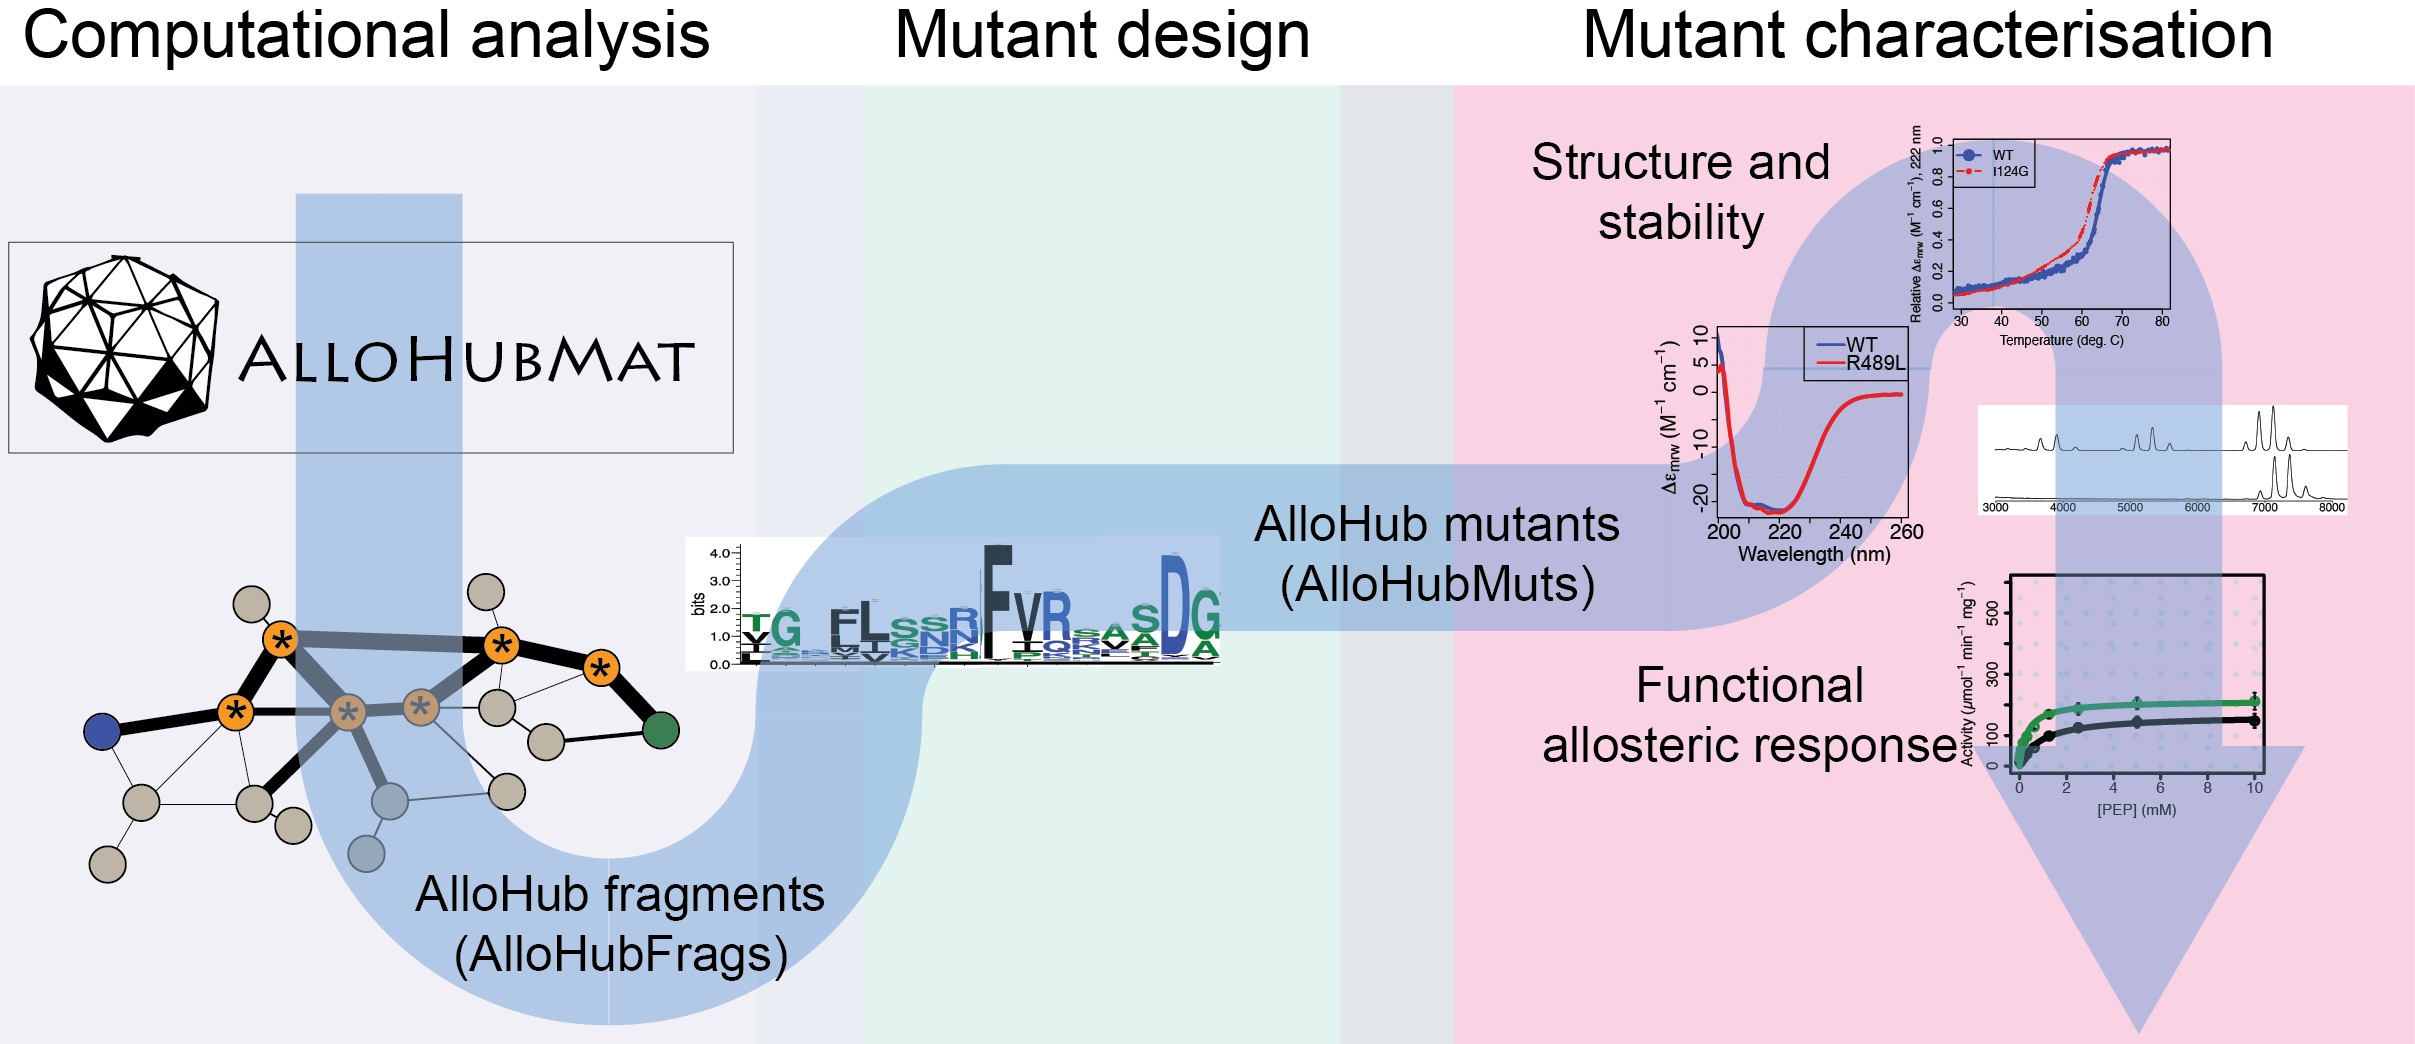
\includegraphics[scale=0.75]{ch7_fig1_schematic.png}
\caption[An integrated computational and experimental strategy for identifying residues which transmit allosteric information between a binding pocket and the active site of a protein. ] {\textbf{An integrated computational and experimental strategy for identifying residues which transmit allosteric information between a binding pocket and the active site of a protein.} AlloHubMat is used to identify candidate allosteric residues, which guide the rational design of allosteric hub mutants (AlloHubMuts). The AlloHubMuts are characterised with a series of experimental methods, in order to interrogate their biophysical and enzymatic response to FBP, Phe and Ser.}
\label{fig:schmatic}
\end{figure}
%
%

\clearpage

\section{Biophysical characterisation of the AlloHubMuts}

\subsection{AlloHubMuts have the same secondary structure content as PKM2(WT)}
Small changes to the local chemical composition of proteins can result in significant conformational changes. Even single-point mutants can affect the stability of proteins, resulting in changes to secondary structural content \cite{Wang:2001aa}. In order to investigate the secondary structure content of the AlloHubMuts and to determine whether the inserted amino acid changes significantly affected the protein fold, far-UV circular dichroism (CD) spectra were acquired for PKM2(WT) and for each of the AlloHubMuts. A superimposition of the AlloHubMut far-UV CD spectra with that of PKM2(WT) revealed very little detectable difference in the shape and intensities of the spectra (\textbf{Fig. \ref{fig:far_uv_cd}}), suggesting that none of the AlloHubMuts appreciably changed the secondary structure content of PKM2. 
%
%
%%% FIGURE
%
\begin{figure}[!ht]
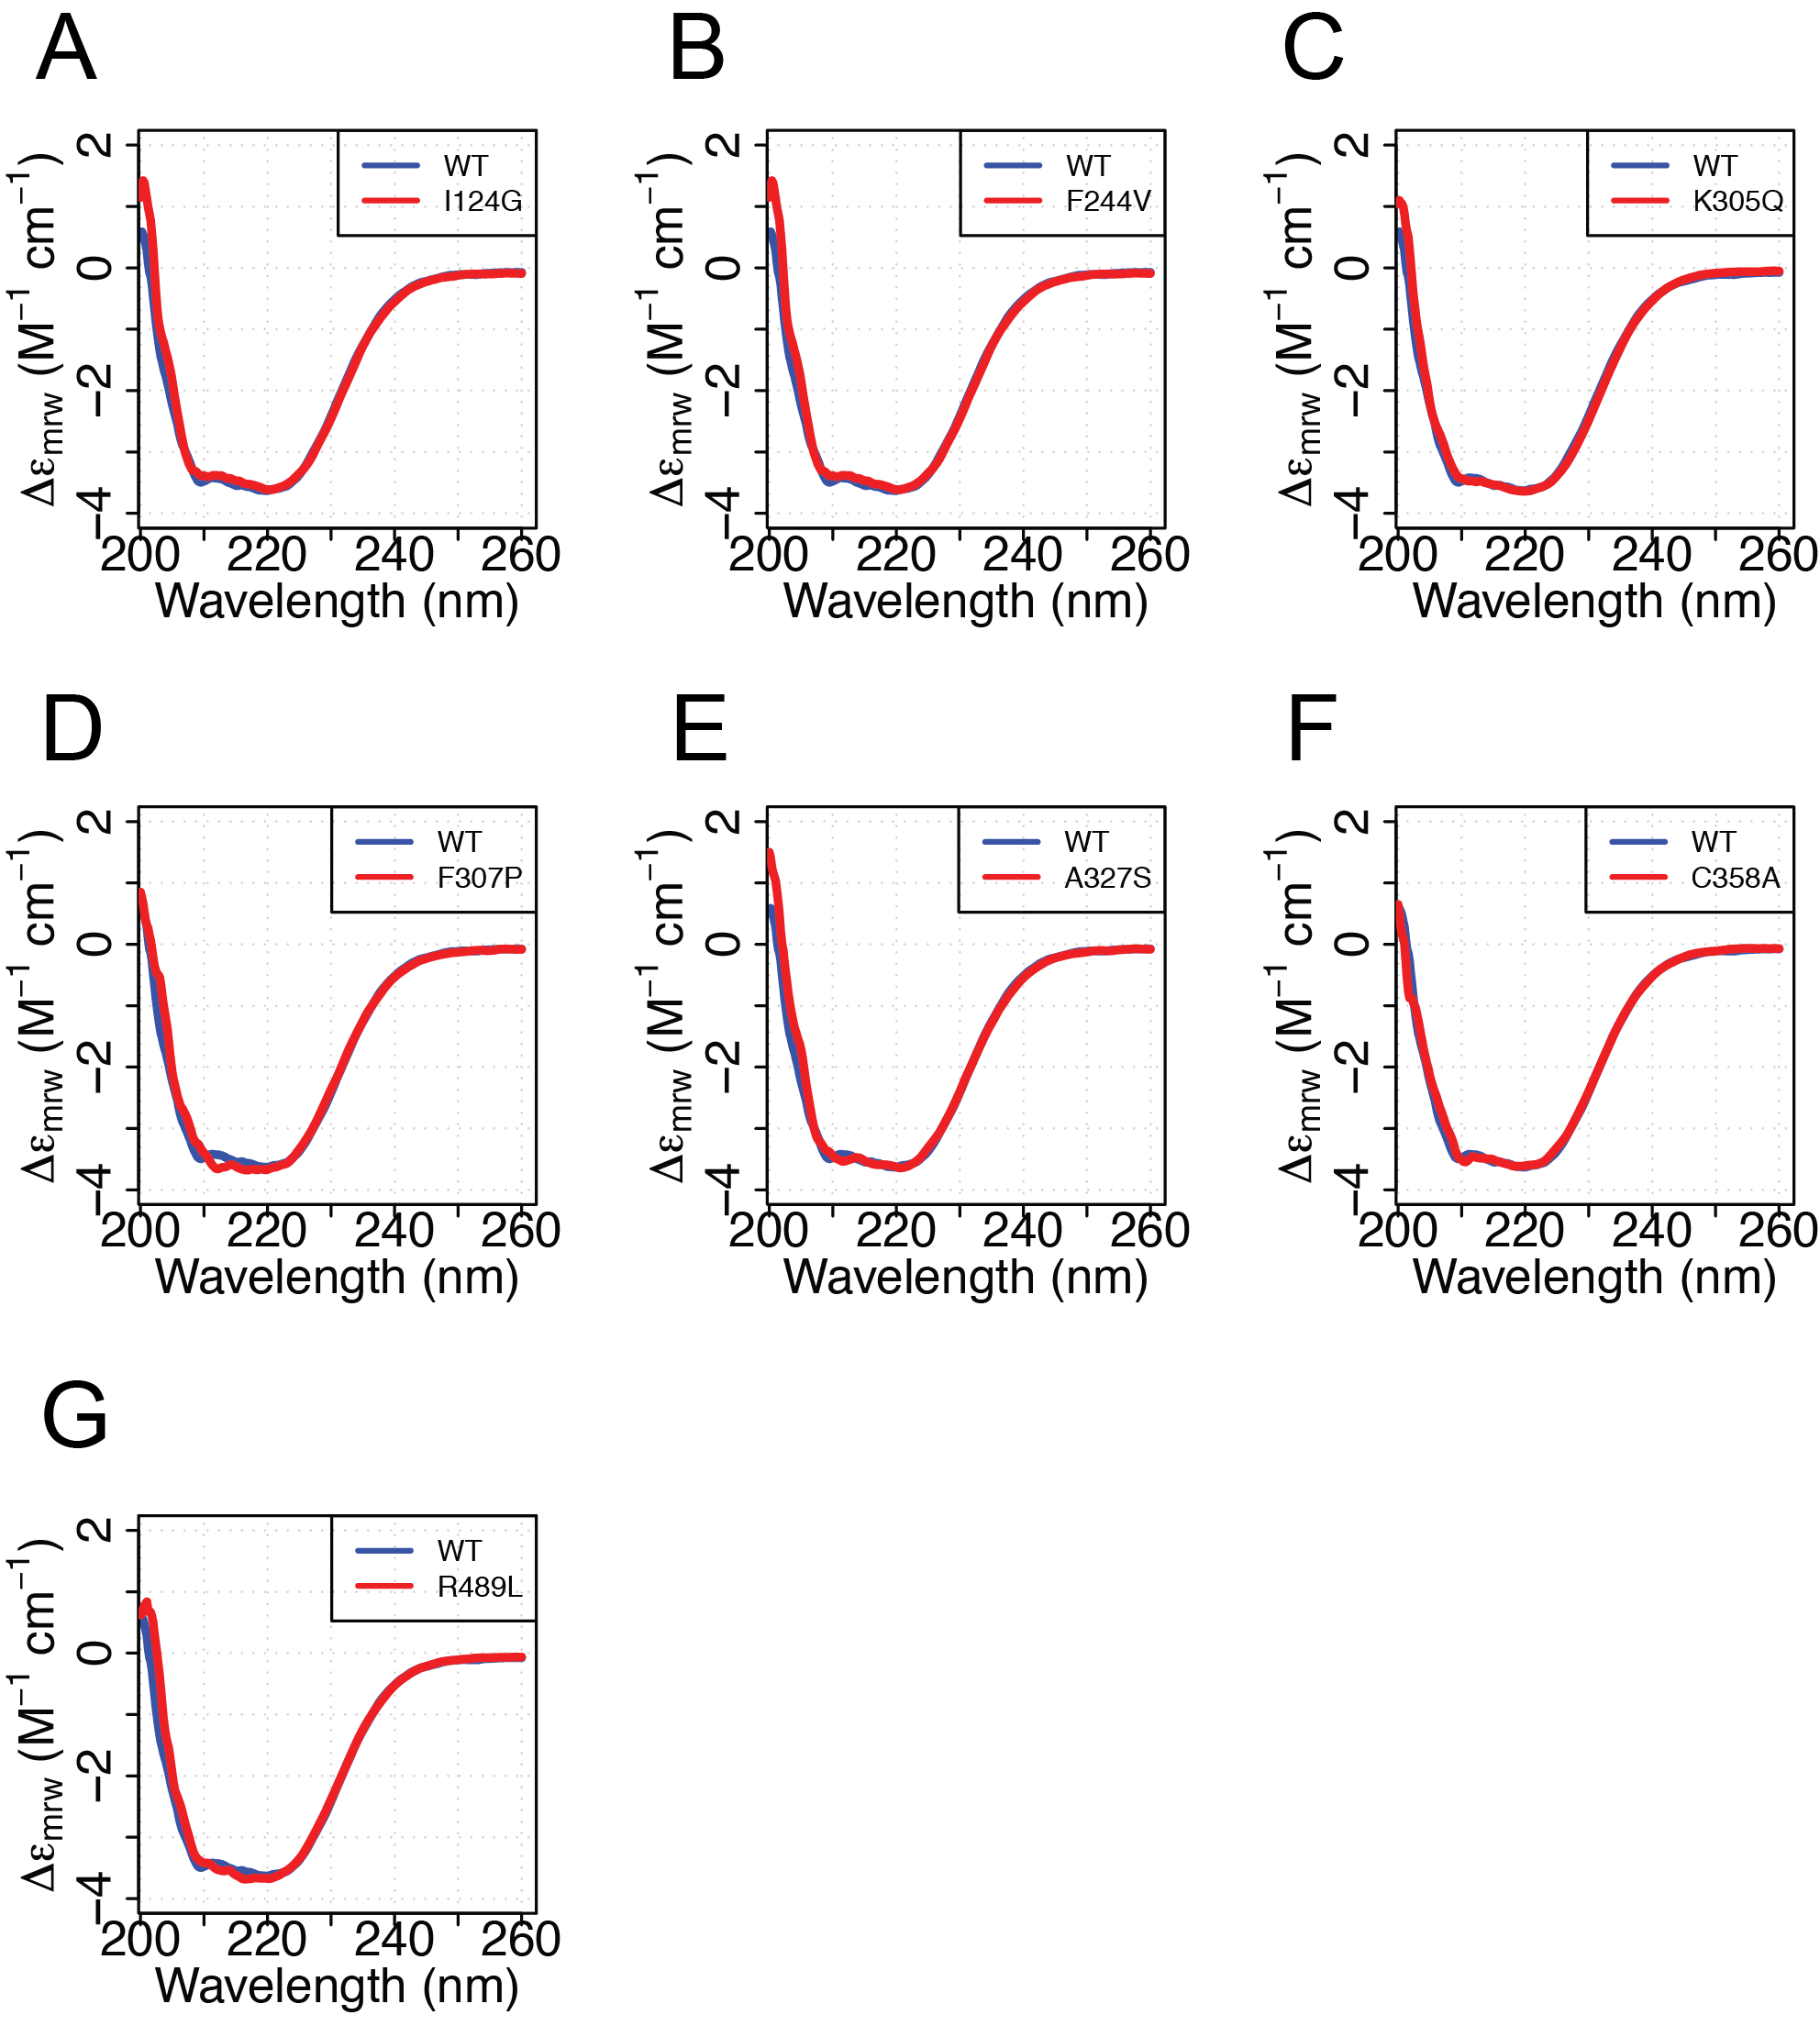
\includegraphics[scale=0.8]{ch7_fig2_far_UV_CD.png}
\caption[Far-UV circular dichroism spectra of AlloHubMuts suggest no change in secondary structure content.] {\textbf{Far-UV circular dichroism spectra of AlloHubMuts suggest no change in secondary structure content.} Far-UV CD spectra of PKM2(WT) and of the seven AlloHubMuts were acquired between 200 nm and 260 nm. Spectra of the AlloHubMuts (red) are superimposed with that of PKM2(WT) (blue); \textbf{(A)} I124G, \textbf{(B)} F244V, \textbf{(C)} K305Q, \textbf{(D)} F307P, \textbf{(E)} A327S, \textbf{(F)} C358A, \textbf{(G)} R489L. A protein concentration of 0.15 mg $\cdot$ mL$^{-1}$ was used in the acquisition of all spectra.}
\label{fig:far_uv_cd}
\end{figure}
%
%
\clearpage

\subsection{AlloHubMuts at either the A-A' or C-C' interfaces show distinct thermodynamics properties}
The far-UV CD spectra of the AlloHubMuts were similar to that of PKM2(WT), suggesting that the mutants did not significantly alter the secondary structure of the protein. Nevertheless, a substantial alteration in secondary structure content would likely be required for changes to become apparent in the far-UV CD spectrum, given the large size of the PKM2 tetramer (234 kDa). Moreover, local conformational changes could conceivably perturb protein stability without enacting changes to the secondary structure content. 
%
%
\\\\
%
%
To this end, thermal unfolding experiments were performed to determine the melting temperature ($T_m$) of each AlloHubMut. PKM2(K305Q) and PKM2(R489L) were found to be thermally destabilising, reflected by a significant decrease in the $T_m$ relative to PKM2(WT) (\textbf{Fig. \ref{fig:unfolding_apo}} and Table \ref{tab:unfolding_kinetics}). None of the other AlloHubMuts were found to have a significant effect on the melting temperature, compared to PKM2(WT) (\textbf{Fig. \ref{fig:unfolding_apo} A-G}). The two destabilising mutants K305Q and R489L are located at subunit interfaces within the PKM2 structure. K305 forms a charged interaction with E384 on the protomer on the opposite side of the A-A' interface (\textbf{Fig. \ref{fig:unfolding_apo} H}). Replacing the $\epsilon$-ammonium group of lysine with an amide group of glutamine caps the side-chain charge and likely prevented the formation of inter-protomeric charged interactions at position 305, possibly reducing oligomer formation and stability of the protein. R489 is positioned proximal to the C-C' interface, though does not form inter-protomeric interactions in the crystal structure of PKM2. Rather, its guanidino group forms charged interactions with the 1'-phosphate group of FBP (\textbf{Fig. \ref{fig:unfolding_apo} I}), and therefore contributes to the binding of FBP. Replacing the guanidino group with an isobutyl group at position 489 likely reducing the binding affinity of FBP.
%
%
\\\\
%
%
Ligand binding can increase a protein's thermal stability because the ligand favours the folded state in the folded-to-unfolded equilibrium. Nevertheless, we consistently found that the addition of saturating concentrations of FBP to PKM2(WT) did not change the melting temperature of the protein (\textbf{Fig. \ref{fig:unfolding_fbp} A}). The lack of FBP-induced thermal stabilisation was likely due to co-purification of PKM2(WT) with endogenous FBP (Section \ref{subsec:fbp_binding_pkm2}). Similarly, I124G, F244V, F307P, A327S and C358A showed no significant changes in their thermal stabilities upon FBP addition (\textbf{Fig. \ref{fig:unfolding_fbp}} and Table \ref{tab:unfolding_kinetics}), suggesting that these variants also retain substoichiometric amounts of endogenous FBP during protein purification.
%
%
\\\\
%
%
The mutation with the largest destabilising effect was PKM2(K305Q), which produced a 19.1 $^\circ$C decrease in the apparent melting temperature and a 174.9 (kJ/mol) decrease in the change in enthalpy at $T_m$, compared to the wild-type. In contrast, the PKM2(R489L) at the C-C' interface produced a comparatively small decrease in the melting temperature (5.6 $^\circ$C). Intriguingly, the thermal stability of the R489L mutant was rescued the $\Delta T_{m}^{WT \rightarrow R489L}$ from 5.6 to 2.4 $^\circ$C - equivalent to wild-type levels (\textbf{Fig. \ref{fig:unfolding_fbp}} and Table \ref{tab:unfolding_kinetics}). In contrast, even when in the presence of 1 mM FBP, PKM2(K305Q) was markedly less stable than the wild-type protein (\textbf{Fig. \ref{fig:unfolding_fbp}} and Table \ref{tab:unfolding_kinetics}).
%
%
\\\\
%
%
Taken together, experimental analyses of the thermal stability of the AlloHubMuts revealed that all AlloHubMuts, with the exception of K305Q and R489L, had similar equilibrium unfolding kinetics as PKM2(WT). Given that the position of R489 is proximal to the FBP binding pocket and the finding that FBP addition rescued the thermal stability of the mutant variant, it is likely that PKM2(R489L) reflects the thermal stability of PKM2 devoid of FBP. Conversely, PKM2(K305Q) is hypothesised to introduce changes to the A-A' interface charged interactions, resulting in protein destabilisation, which is not rescued by FBP addition. 
%
%
%%% TABLE
\begin{table}[hbt]
\centering
\caption[Equilibrium thermal unfolding kinetic parameters of the AlloHubMuts.] {\textbf{Equilibrium thermal unfolding kinetic parameters of the AlloHubMuts.} A two-phase unfolding model (Methods Section \ref{methods:cd_spec}) was fit to each of the unfolding curves shown in \textbf{Fig. \ref{fig:unfolding_apo}}. The change in enthalpy ($\Delta$H ) and entropy ($\Delta$S) between the folded and semi-unfolded states, as well as the melting temperature ($T_{m}$) is reported.}
\label{tab:unfolding_kinetics}
\begin{tabular}{@{}llll@{}}
\toprule
PKM2 variant & $\Delta$H (kJ/mol) 		& $\Delta$S (kJ/K $\cdot$ mol) & $T_{m}$ ($^\circ$C) \\ \midrule
WT        					&  525.8 $\pm$  44.8        &         8.2   $\pm$  0.7               &      63.9 $\pm$  0.1       \\
WT + 1 mM FBP      &  492.4 $\pm$  23.6        &         7.8   $\pm$  0.4               &      63.1 $\pm$  0.1       \\ \midrule
I124G    					&  336.5  $\pm$ 23. 1        &         5.4   $\pm$ 0.4                &     	61.3  $\pm$  0.1       \\
I124G + 1 mM FBP 	&  600.0  $\pm$ 22.6        &         9.8  $\pm$ 0.4                &     	61.3  $\pm$  0.4       \\ \midrule
F244V   					&  477.2  $\pm$ 16.9         &         7.6  $\pm$ 0.3                 &      62.5 $\pm$ 0.1        \\ 
F244V + 1 mM FBP 	&  525.0  $\pm$ 34.5         &         8.6  $\pm$ 0.6                &      61.3 $\pm$ 0.1        \\ \midrule
K305Q  					&  350.9  $\pm$ 13.5        &         7.8  $\pm$ 0.3                 &      44.8 $\pm$ 0.1        \\ 
K305Q + 1 mM FBP   &  479.5  $\pm$ 20.9        &         8.7 $\pm$ 0.4                 &      54.8 $\pm$ 0.1        \\ \midrule
F307P   					&  477.8  $\pm$ 18.2        &         7.7 $\pm$ 0.3                 &      62.3 $\pm$ 0.1        \\ 
F307P + 1 mM FBP	&  695.2  $\pm$ 36.2        &         11.3 $\pm$ 0.6                 &      61.7 $\pm$ 0.1        \\ \midrule
A327S   					&  558.2  $\pm$ 14.8        &         9.2 $\pm$ 0.2                 &      60.8 $\pm$ 0.4        \\ 
A327S + 1 mM FBP	&  653.4  $\pm$ 40.8        &         10.9 $\pm$ 0.7                 &      59.9 $\pm$ 0.1        \\ \midrule
C358A   					&  493.9  $\pm$ 20.1        &         7.9 $\pm$ 0.3                 &      62.7 $\pm$ 0.1        \\
C358A + 1 mM FBP &  660.4  $\pm$ 22.2        &         11.0 $\pm$ 0.4                 &      60.3 $\pm$ 0.1        \\ \midrule
K433E  						&  488.4  $\pm$ 9.6         &         5.1 $\pm$ 0.2                 &      56.8 $\pm$ 0.1        \\ 
K433E + 1 mM FBP	&  678.0  $\pm$ 27.6         &         11.6 $\pm$ 0.5                &      58.1 $\pm$ 0.1        \\ \midrule
R489L  						&  232.9  $\pm$ 21.4         &         4.0 $\pm$ 0.4                 &      58.2 $\pm$ 0.3        \\
R489L + 1 mM FBP  &  643.3  $\pm$ 45.6         &         10.5 $\pm$ 0.7                 &      61.5 $\pm$ 0.1        \\ \bottomrule
\end{tabular}
\end{table}
%
%
%
%
%
%%% FIGURE
%
\begin{figure}[!ht]
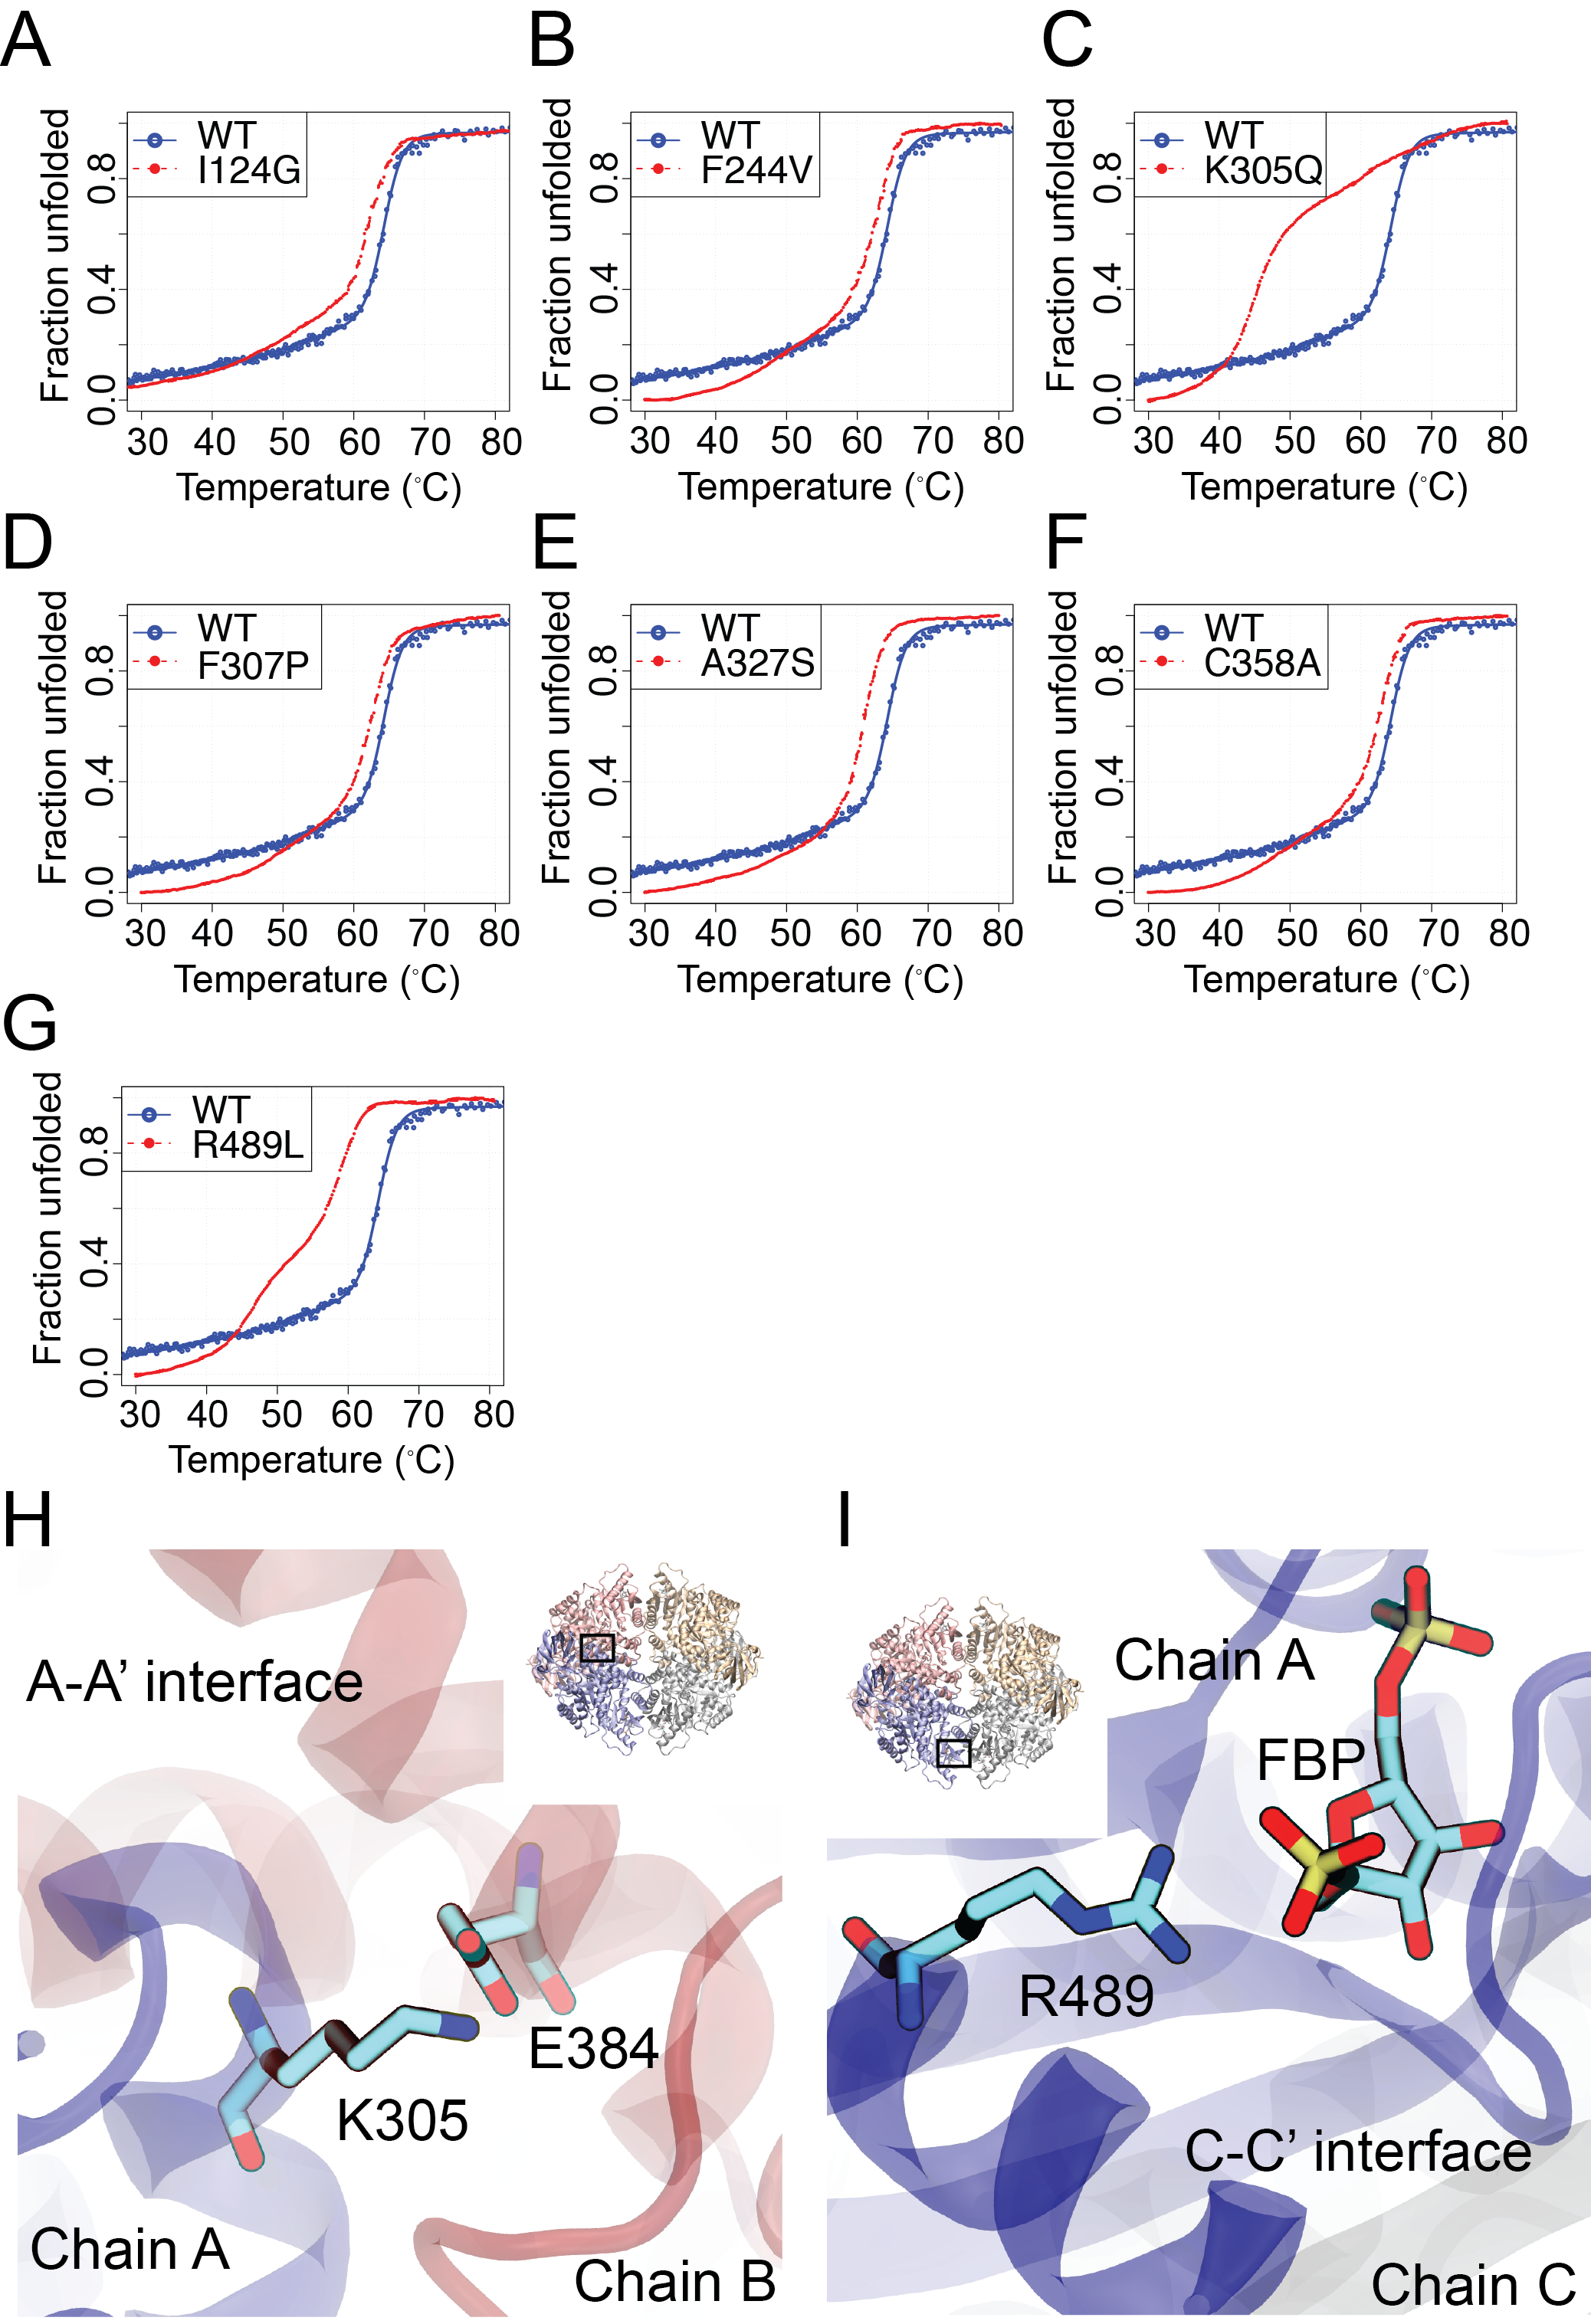
\includegraphics[scale=0.7]{ch7_fig3_unfolding_apo.png}
\caption[Thermal unfolding spectra of the AlloHubMuts fitted to a two-phase unfolding model.] {\textbf{Thermal unfolding spectra of the AlloHubMuts fitted to a two-phase unfolding model.} \textbf{(A-G)} Far-UV CD intensity at 222 nm of PKM2(WT) (blue) and the AlloHubMuts (red) were monitored over a range of temperatures between 30 \textdegree C and 80 \textdegree C, in the absence of any added ligands. Data points were fitted to a two-phase unfolding curve. \textbf{(H)} A schematic of the local structure of K305 at the A-A' interface and \textbf{(I)} R489 at the FBP binding pocket.}
\label{fig:unfolding_apo}
\end{figure}
%
%
\clearpage

%
%
%
%
%
%%% FIGURE
%
\begin{figure}[!ht]
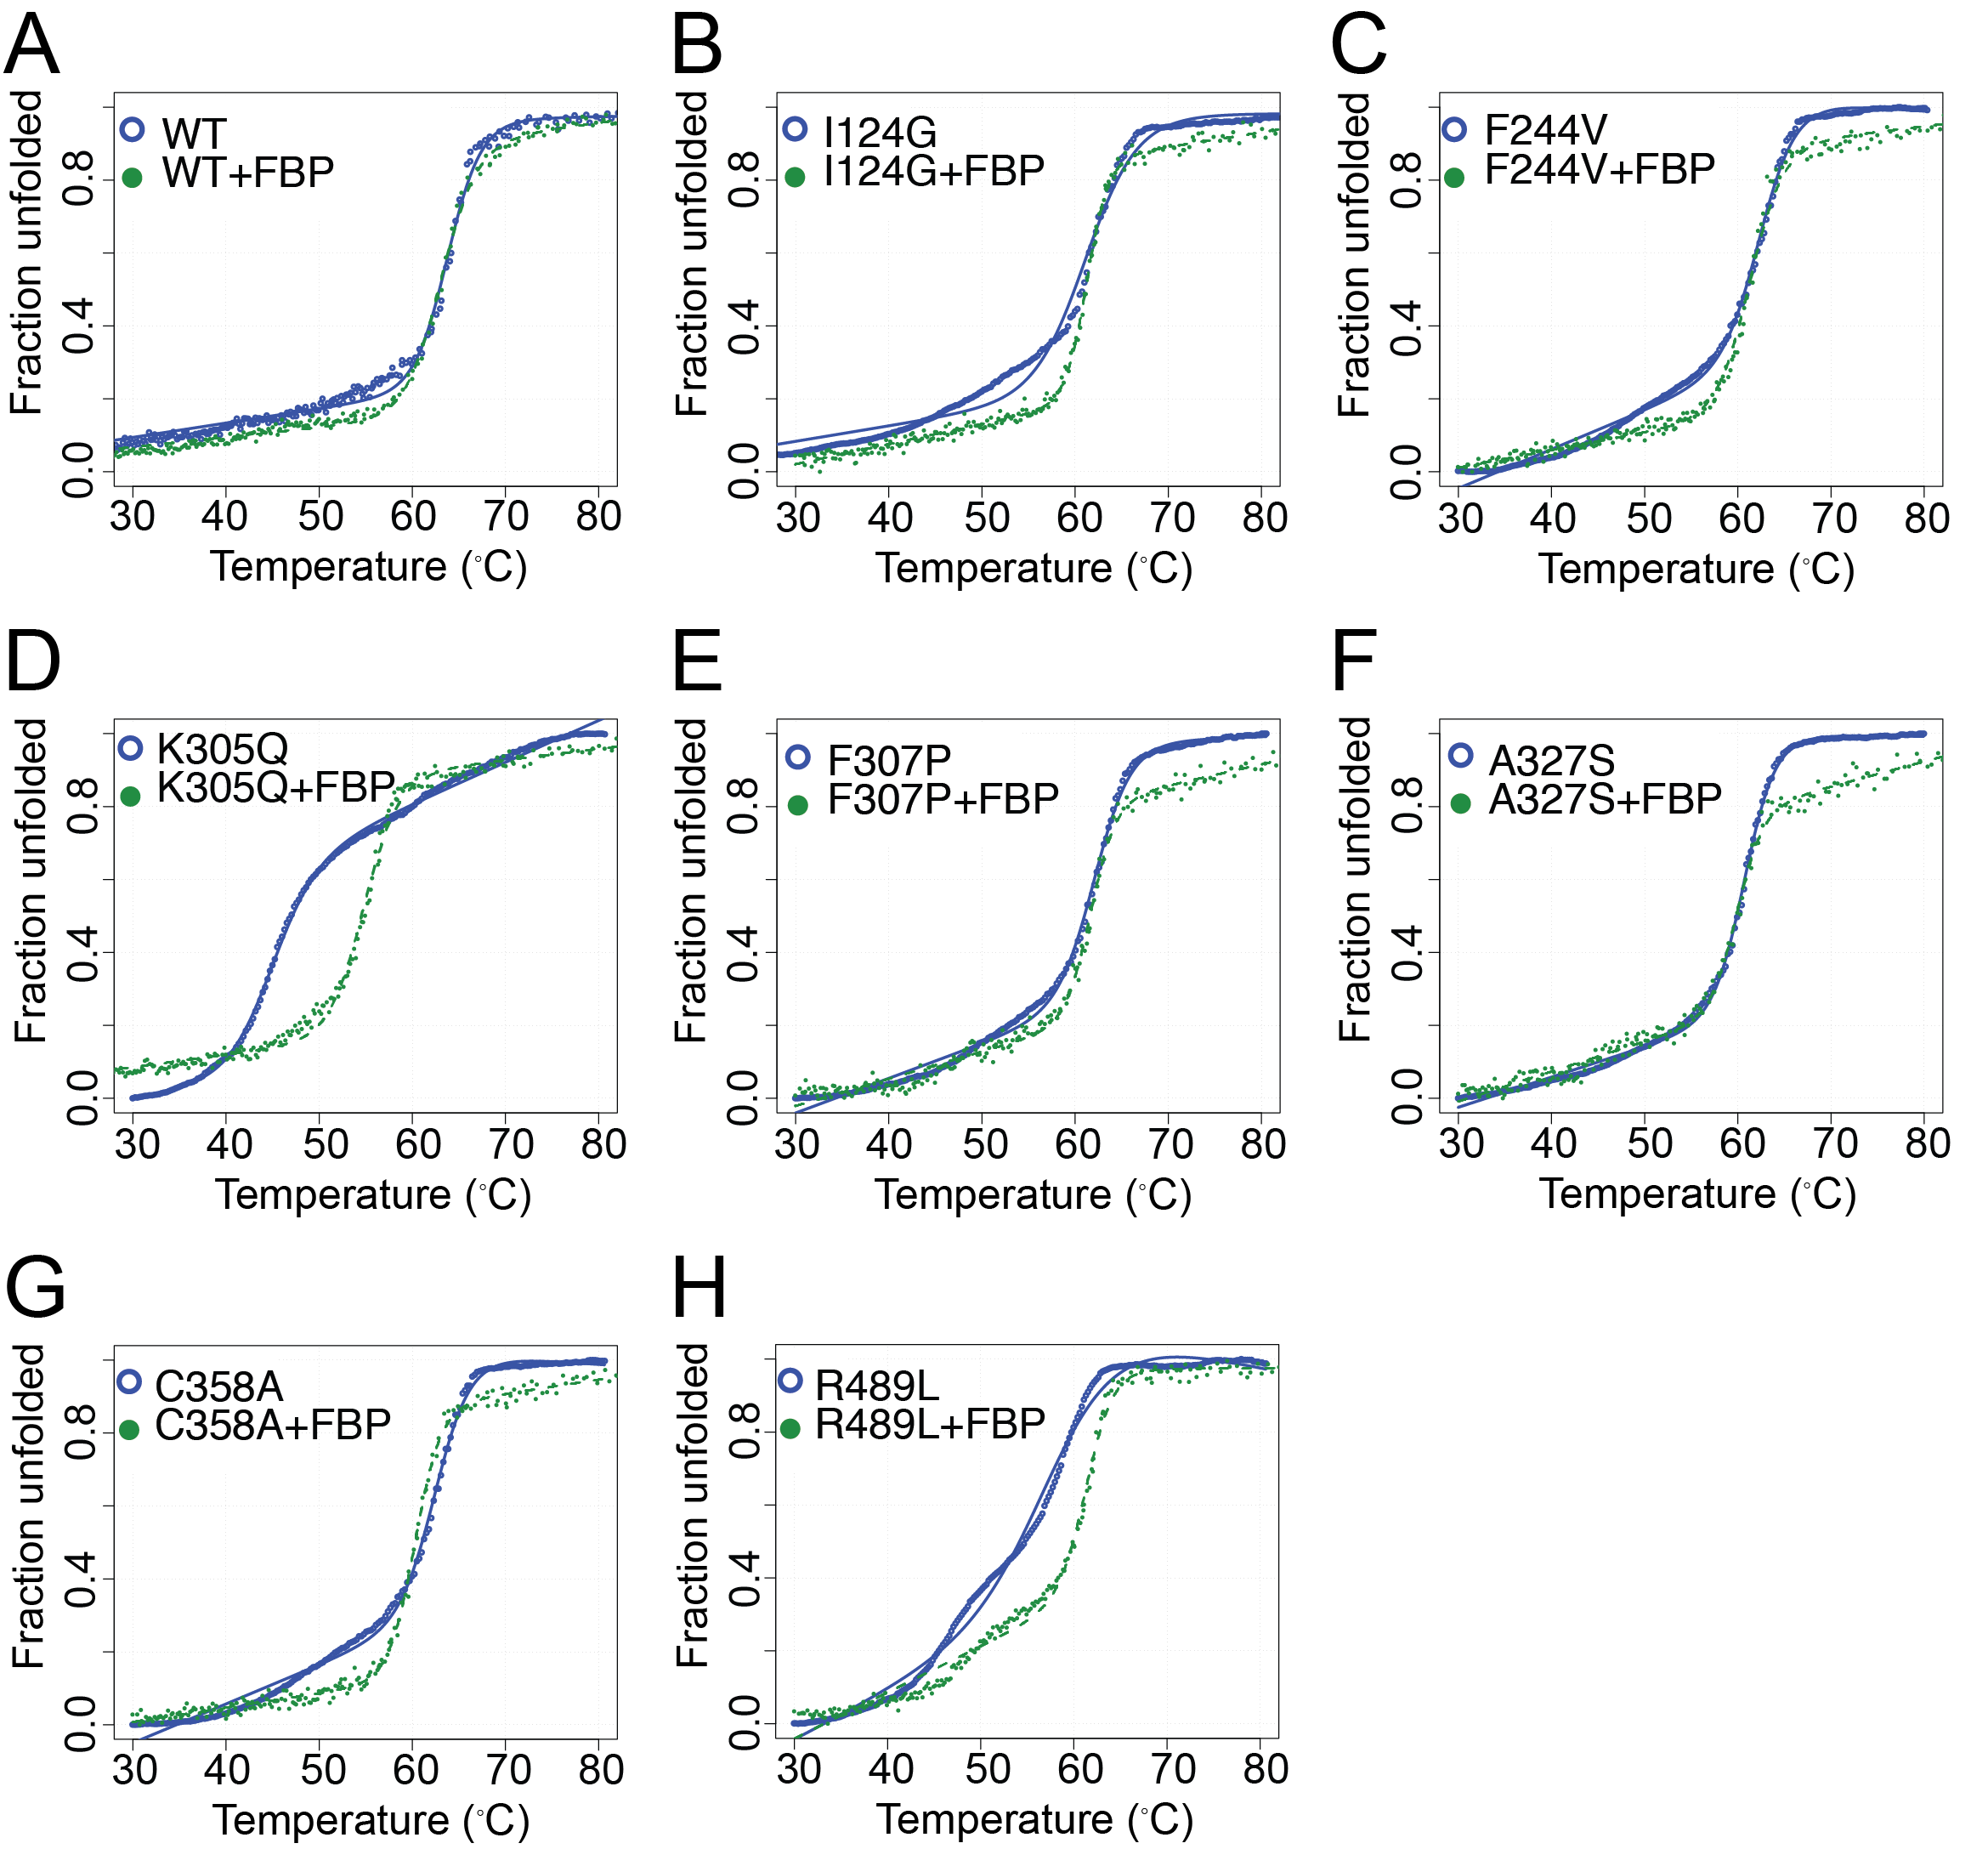
\includegraphics[scale=0.7]{ch7_fig4_unfolding_fbp.png}
\caption[The thermal stability of PKM2(K305Q) and PKM2(R489L) is increased upon FBP addition.] {\textbf{The thermal stability of PKM2(K305Q) and PKM2(R489L) is increased upon FBP addition.} Far-UV CD intensity at 222 nm was monitored for \textbf{(A)} PKM2(WT) and \textbf{(B-H)} the AlloHubMuts in the absence (blue) and in the presence (green) of 1 mM FBP.}
\label{fig:unfolding_fbp}
\end{figure}
%
%
\clearpage

\subsection{R489L reduces the binding affinity to FBP}
The reduced thermal stability of PKM2(R489L) and the fact that R489 forms a charge-charge interaction with the 1'-phosphate group of FBP, suggested that this mutant may have a reduced FBP binding affinity. Binding affinities of the AlloHubMuts to FBP (Table \ref{tab:fbp_binding_allohubmuts}) were calculated from fluorescence titration measurements (\textbf{Fig. \ref{fig:fbp_binding_allohubmuts} A-G}), as previously described (Section \ref{subsec:fbp_binding_pkm2}). All of the AlloHubMuts bound to FBP with nano molar affinity, with the exception of PKM2(R489L), which was estimated to bind to FBP with an apparent affinity of (14.0 $\pm$ 2.7) mM. Despite the two-order of magnitude decrease in the apparent binding affinity of PKM2(R489L) for FBP, ligand binding saturated the measured tryptophan fluorescence changes at mM concentrations (\textbf{Fig. \ref{fig:fbp_binding_allohubmuts} G}). 
%
%
%
%%%TABLE
%
% Please add the following required packages to your document preamble:
% \usepackage{booktabs}
\begin{table}[ht]
\centering
\caption[Steady-state dissociation constants of the AlloHubMuts for FBP.] {\textbf{Steady-state dissociation constants of the AlloHubMuts for FBP.} A 1:1 stoichiometry binding curve (\ref{subsec:fbp_binding_pkm2}) was fit to the binding curves in \textbf{Fig. \ref{fig:fbp_binding_allohubmuts}}. The $K_{D}^{FBP}$ is reported in variable units.}
\label{tab:fbp_binding_allohubmuts}
\begin{tabular}{@{}ll@{}}
\toprule
PKM2  & $K_{D}^{FBP}$       \\ \midrule
WT    & (21.4 $\pm$ 9.0) nM  \\
I124G & (39.5 $\pm$ 33.5) nM \\
F244V & (30.7 $\pm$ 33.1) nM \\
K305Q & (39.4 $\pm$ 34.1) nM \\
F307P & (4.0 $\pm$ 12.8) nM  \\
A327S & (43.2 $\pm$ 48.7) nM \\
C358A & (35.3 $\pm$ 23.6) nM \\
R489L & (14.0 $\pm$ 2.7) mM  \\ \bottomrule
\end{tabular}
\end{table}
%
%
%
%
%%% FIGURE
%
\begin{figure}[!ht]
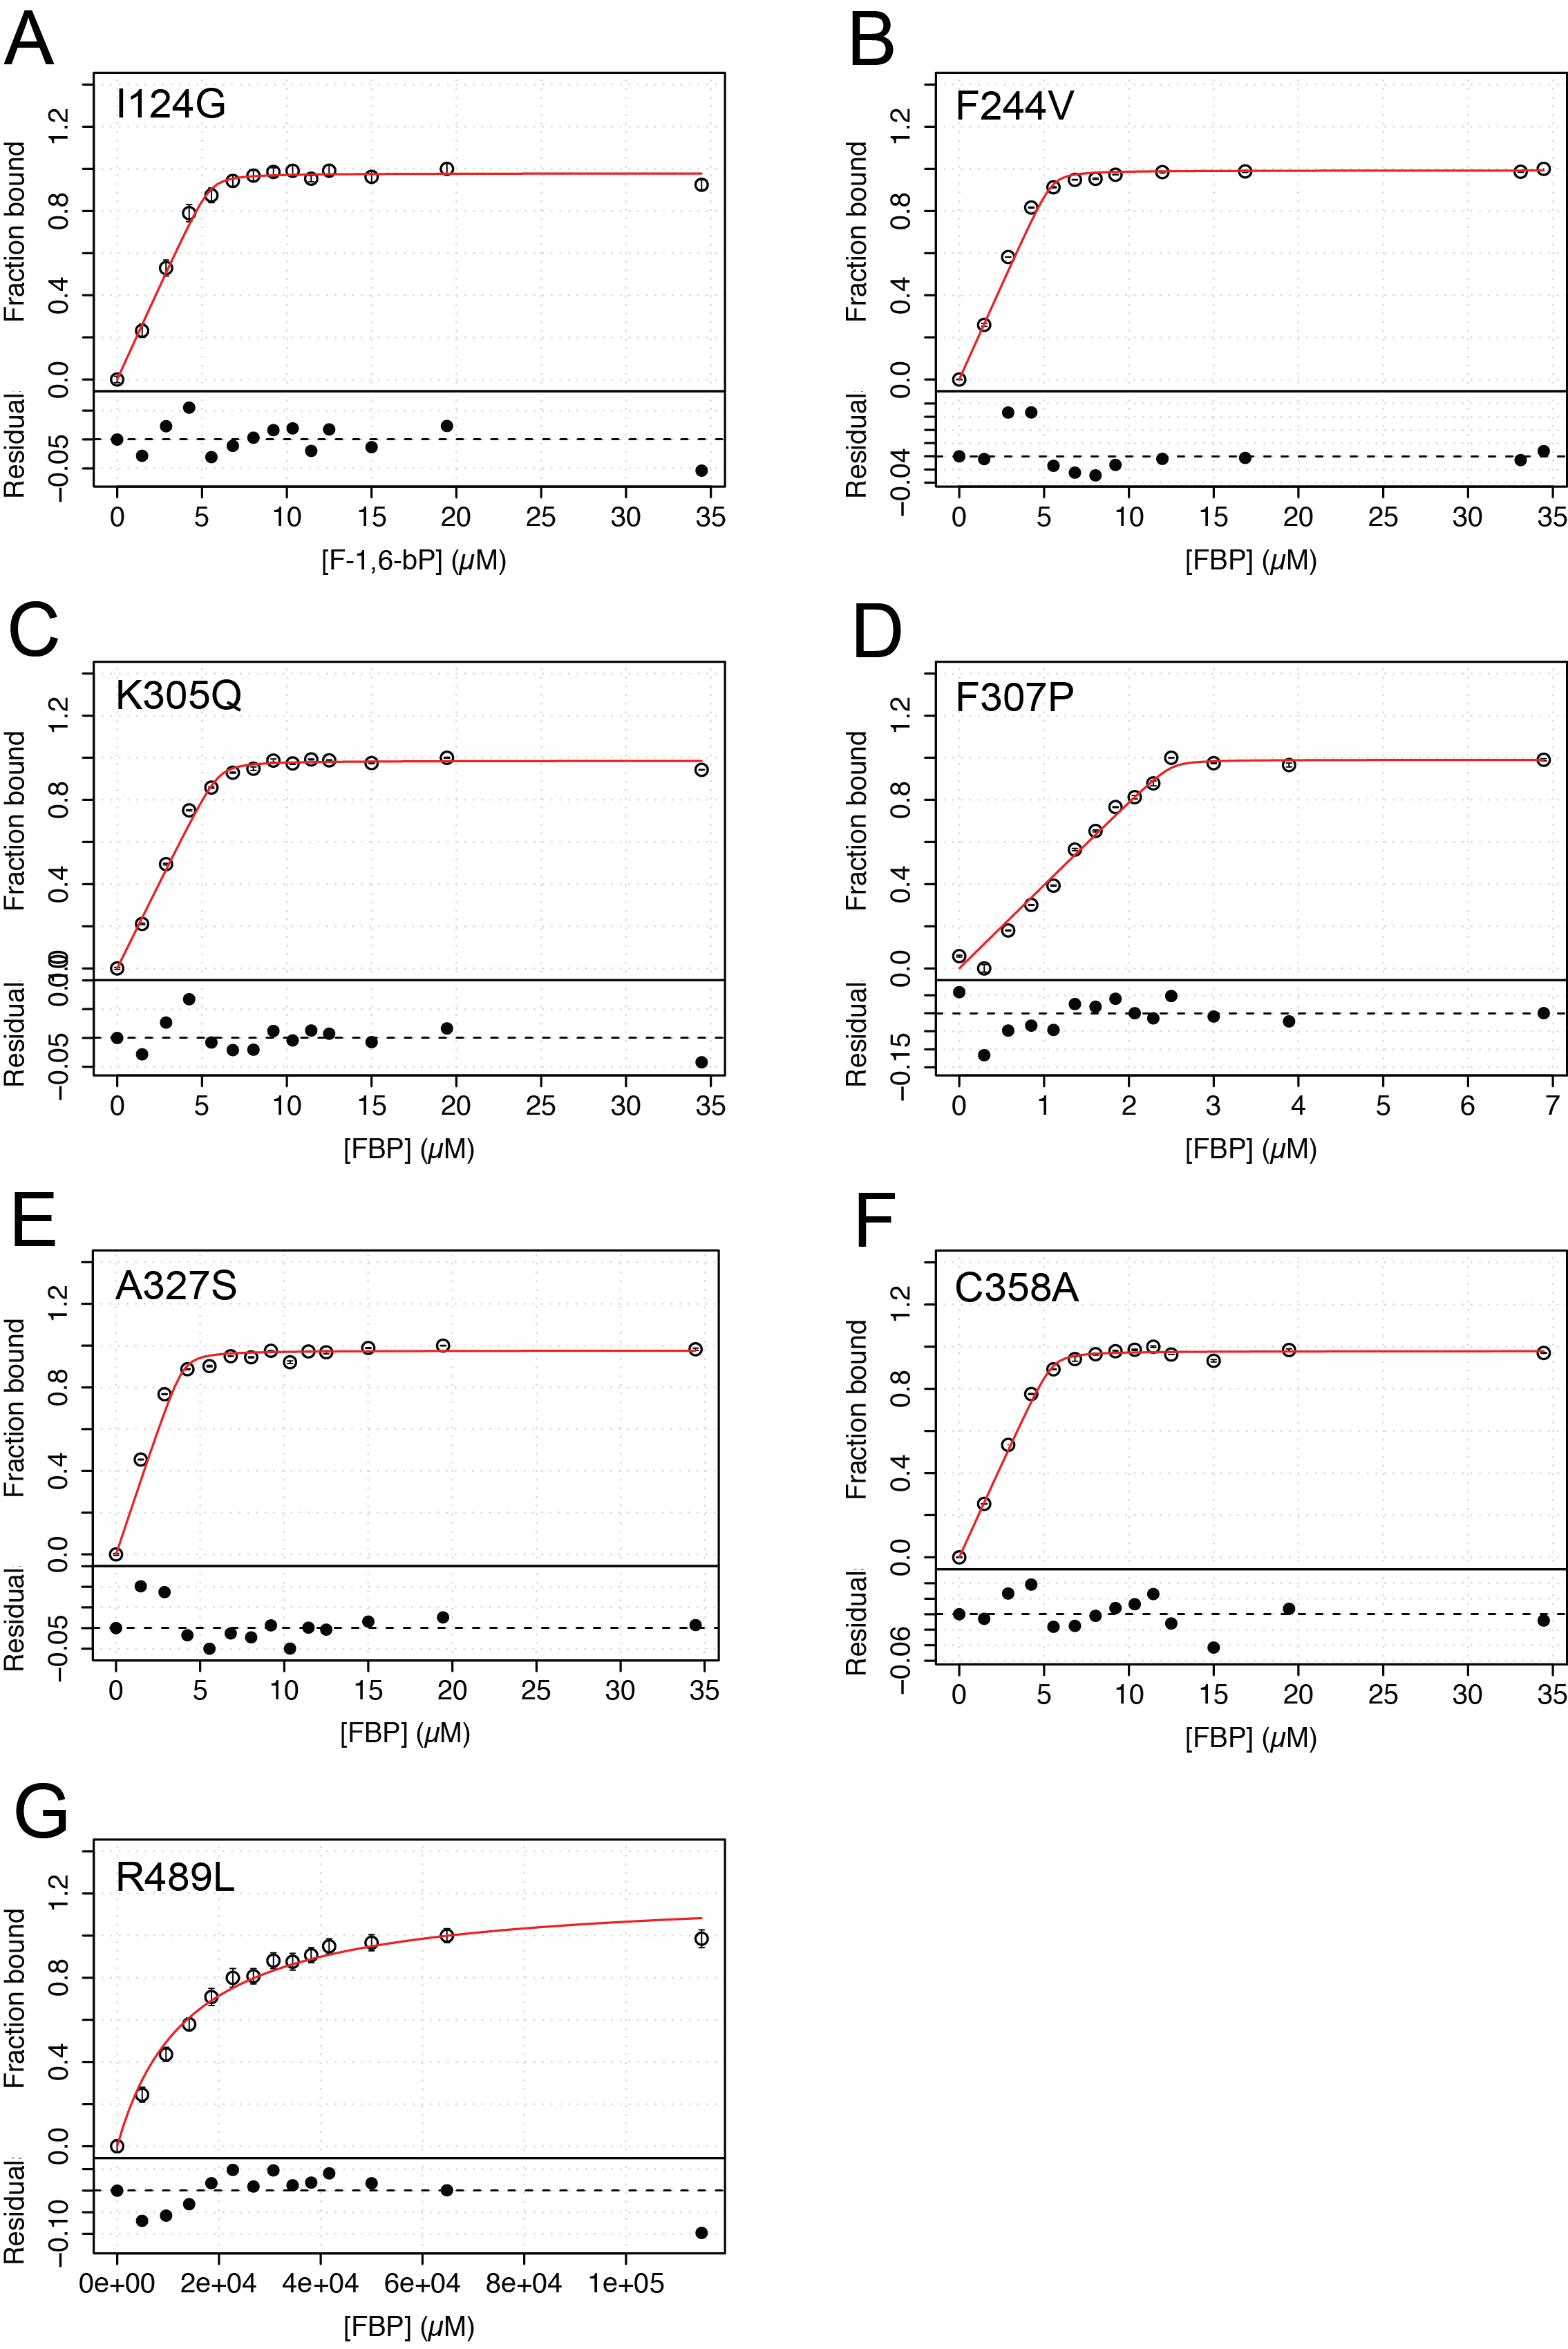
\includegraphics[scale=0.65]{ch7_fig5_fbp_binding.png}
\caption[The AlloHubMuts have a nano molar affinity for FBP with the exception of PKM2(R489L).] {\textbf{The AlloHubMuts have a nano molar affinity for FBP with the exception of PKM2(R489L).} The ratio of the fluorescence emission intensity at 325 nm and 350 nm were recorded over a range of FBP concentrations. Apparent binding curves were fit assuming a 1:1 stoichiometry (red). }
\label{fig:fbp_binding_allohubmuts}
\end{figure}
%
%
\clearpage


\section{Characterisation of the functional response of AlloHubMuts to allosteric ligands}
The AlloHubMuts were identified by the software AlloHubMat as candidate residues, which coordinated the allosteric effect of FBP. It was postulated that changing the chemical composition of these residues would perturb the allosteric coupling between the FBP binding pocket and the active site. To test this hypothesis we sought to characterise the steady-state enzyme kinetics of each AlloHubMut and the activity response of each mutant to the addition of FBP. 

\subsection{Several AlloHubMuts attenuate the allosteric coupling between the FBP pocket and the active site}
\label{subsec:allohubmuts_fbp}
To assess the functional effect of perturbing the \textit{in silico}-determined allosteric pathways, we measured the steady-state kinetics of the AlloHubMuts in the absence and in the presence of saturating concentrations of FBP. Initial velocity curves were determined over a range of concentrations of phosphoenolpyruvate and revealed that all of the AlloHubMuts had a lower apparent maximal velocity, compared to PKM2(WT), in the absence of FBP (Table \ref{tab:allohubmut_activity}). The addition of FBP resulted in a marked increase in the apparent maximal velocity of PKM2(I124G) and PKM2(R489L) (Table \ref{tab:allohubmut_activity}). PKM2(K305Q) was inactive, both in the absence and in the presence of FBP, suggesting that this AlloHubMut was catalytically dead (Table \ref{tab:allohubmut_activity}). In contrast, PKM2(F307P) appeared to be constitutively active, with a low apparent $K_{M}^{PEP}$, which was unchanged upon FBP addition (Table \ref{tab:allohubmut_activity}).
%
%
\\\\
%
%
As described previously in Chapter \ref{chapter:enzyme_kinetics}, FBP was found to exert its functional allosteric effect on PKM2(WT) by increasing the enzyme-substrate affinity, without changing the maximal velocity. It was therefore postulated that allosteric activation results from a coupling between FBP and PEP binding, mediated by the AlloHub residues (\textbf{Fig. \ref{fig:fbp_coupling_constant} A}). Consequently, we sought to quantitatively determine the coupling between the FBP pocket and the active site for PKM2(WT) and each of the AlloHubMuts, to discern whether, and to which extent, mutations along the predicted FBP pathway perturbed the allosteric coupling.
%
%
\\\\
%
%
Assuming a single-substrate-single-modifier mechanism of PKM2 catalysis (\textbf{Fig. \ref{fig:fbp_coupling_constant} B}), the coupling between the allosteric pocket and the substrate binding site was determined by calculating the log-fold ratio of the Michaelis-Menten constant of the protein saturated with FBP ($K_{M}^{0}$), divided by Michaelis-Menten constant in the absence of FBP ($K_{M}^{X}$) \cite{Reinhart:2004aa}:
%
%
\begin{equation}
Q = \left( \frac{\alpha K_{S}}{K_{S}} \right)
\end{equation}
%
%
A $log \: Q>0$ indicates a positive coupling (activation) and $log \: Q<0$ negative coupling (inhibition). AlloHubMuts I124G, F244V, K305Q, F307P and R489L were all found to show attenuated allosteric coupling between the active site and the FBP pocket compared to PKM2(WT) (\textbf{Fig. \ref{fig:fbp_coupling_constant} C}), indicating that \textit{AlloHubMat} identified residues that mediate the allosteric effect of FBP. In contrast, AlloHubMuts A327S and C358A both had a coupling co-efficient ($Q$), which was unchanged from that of WT, suggesting either that the amino acid substitutions were functionally neutral, or that these residues are not required for FBP-induced activation.


\subsection{AlloHub residues A327 and C358 mediate multi-ligand allosteric coupling}
\label{subsec:allohubmuts_phe}
Previous work presented in Chapters \ref{chapter:enzyme_kinetics} and \ref{chapter:mass_spec}, found that the allosteric inhibitor phenylalanine (Phe) acts to reduce the activating effect of FBP through a functional cross-talk. We sought to investigate whether AlloHubMuts, which abrogated FBP-induced allostery, also perturbed the cross-talk between FBP and Phe. 
%
%
\\\\
%
%
To this end, the coupling co-efficient was measured for the doubly liganded $PKM2^{FBP+Phe}$ state ($Q^{FBP+Phe}$). AlloHubMuts I124G, F244V and R489L revealed the same $Q^{FBP+Phe}$ as the wild-type variant (\textbf{Fig. \ref{fig:fbp_coupling_constant} D}), suggesting either that the allosteric coupling between FBP, Phe and the active site was unchanged for these mutant substitutions, or that residues I124, F244 and R489 do not contribute to the FBP-Phe cross-talk. 
%
%
\\\\
%
%
In contrast, the simultaneous addition of FBP and Phe failed to produce an allosteric response for AlloHubMuts K305Q and F307P (\textbf{Fig. \ref{fig:fbp_coupling_constant} D}), further suggesting that these variants are allosterically inert. Moreover, the addition of Phe to A327S and C358, failed to attenuate FBP-induced activation of these AlloHubMuts, indicating that residues A327 and C358 have a role in coupling the allosteric effect of Phe with that of FBP.
%
%
%
%
%
%%% FIGURE
%
\begin{figure}[!ht]
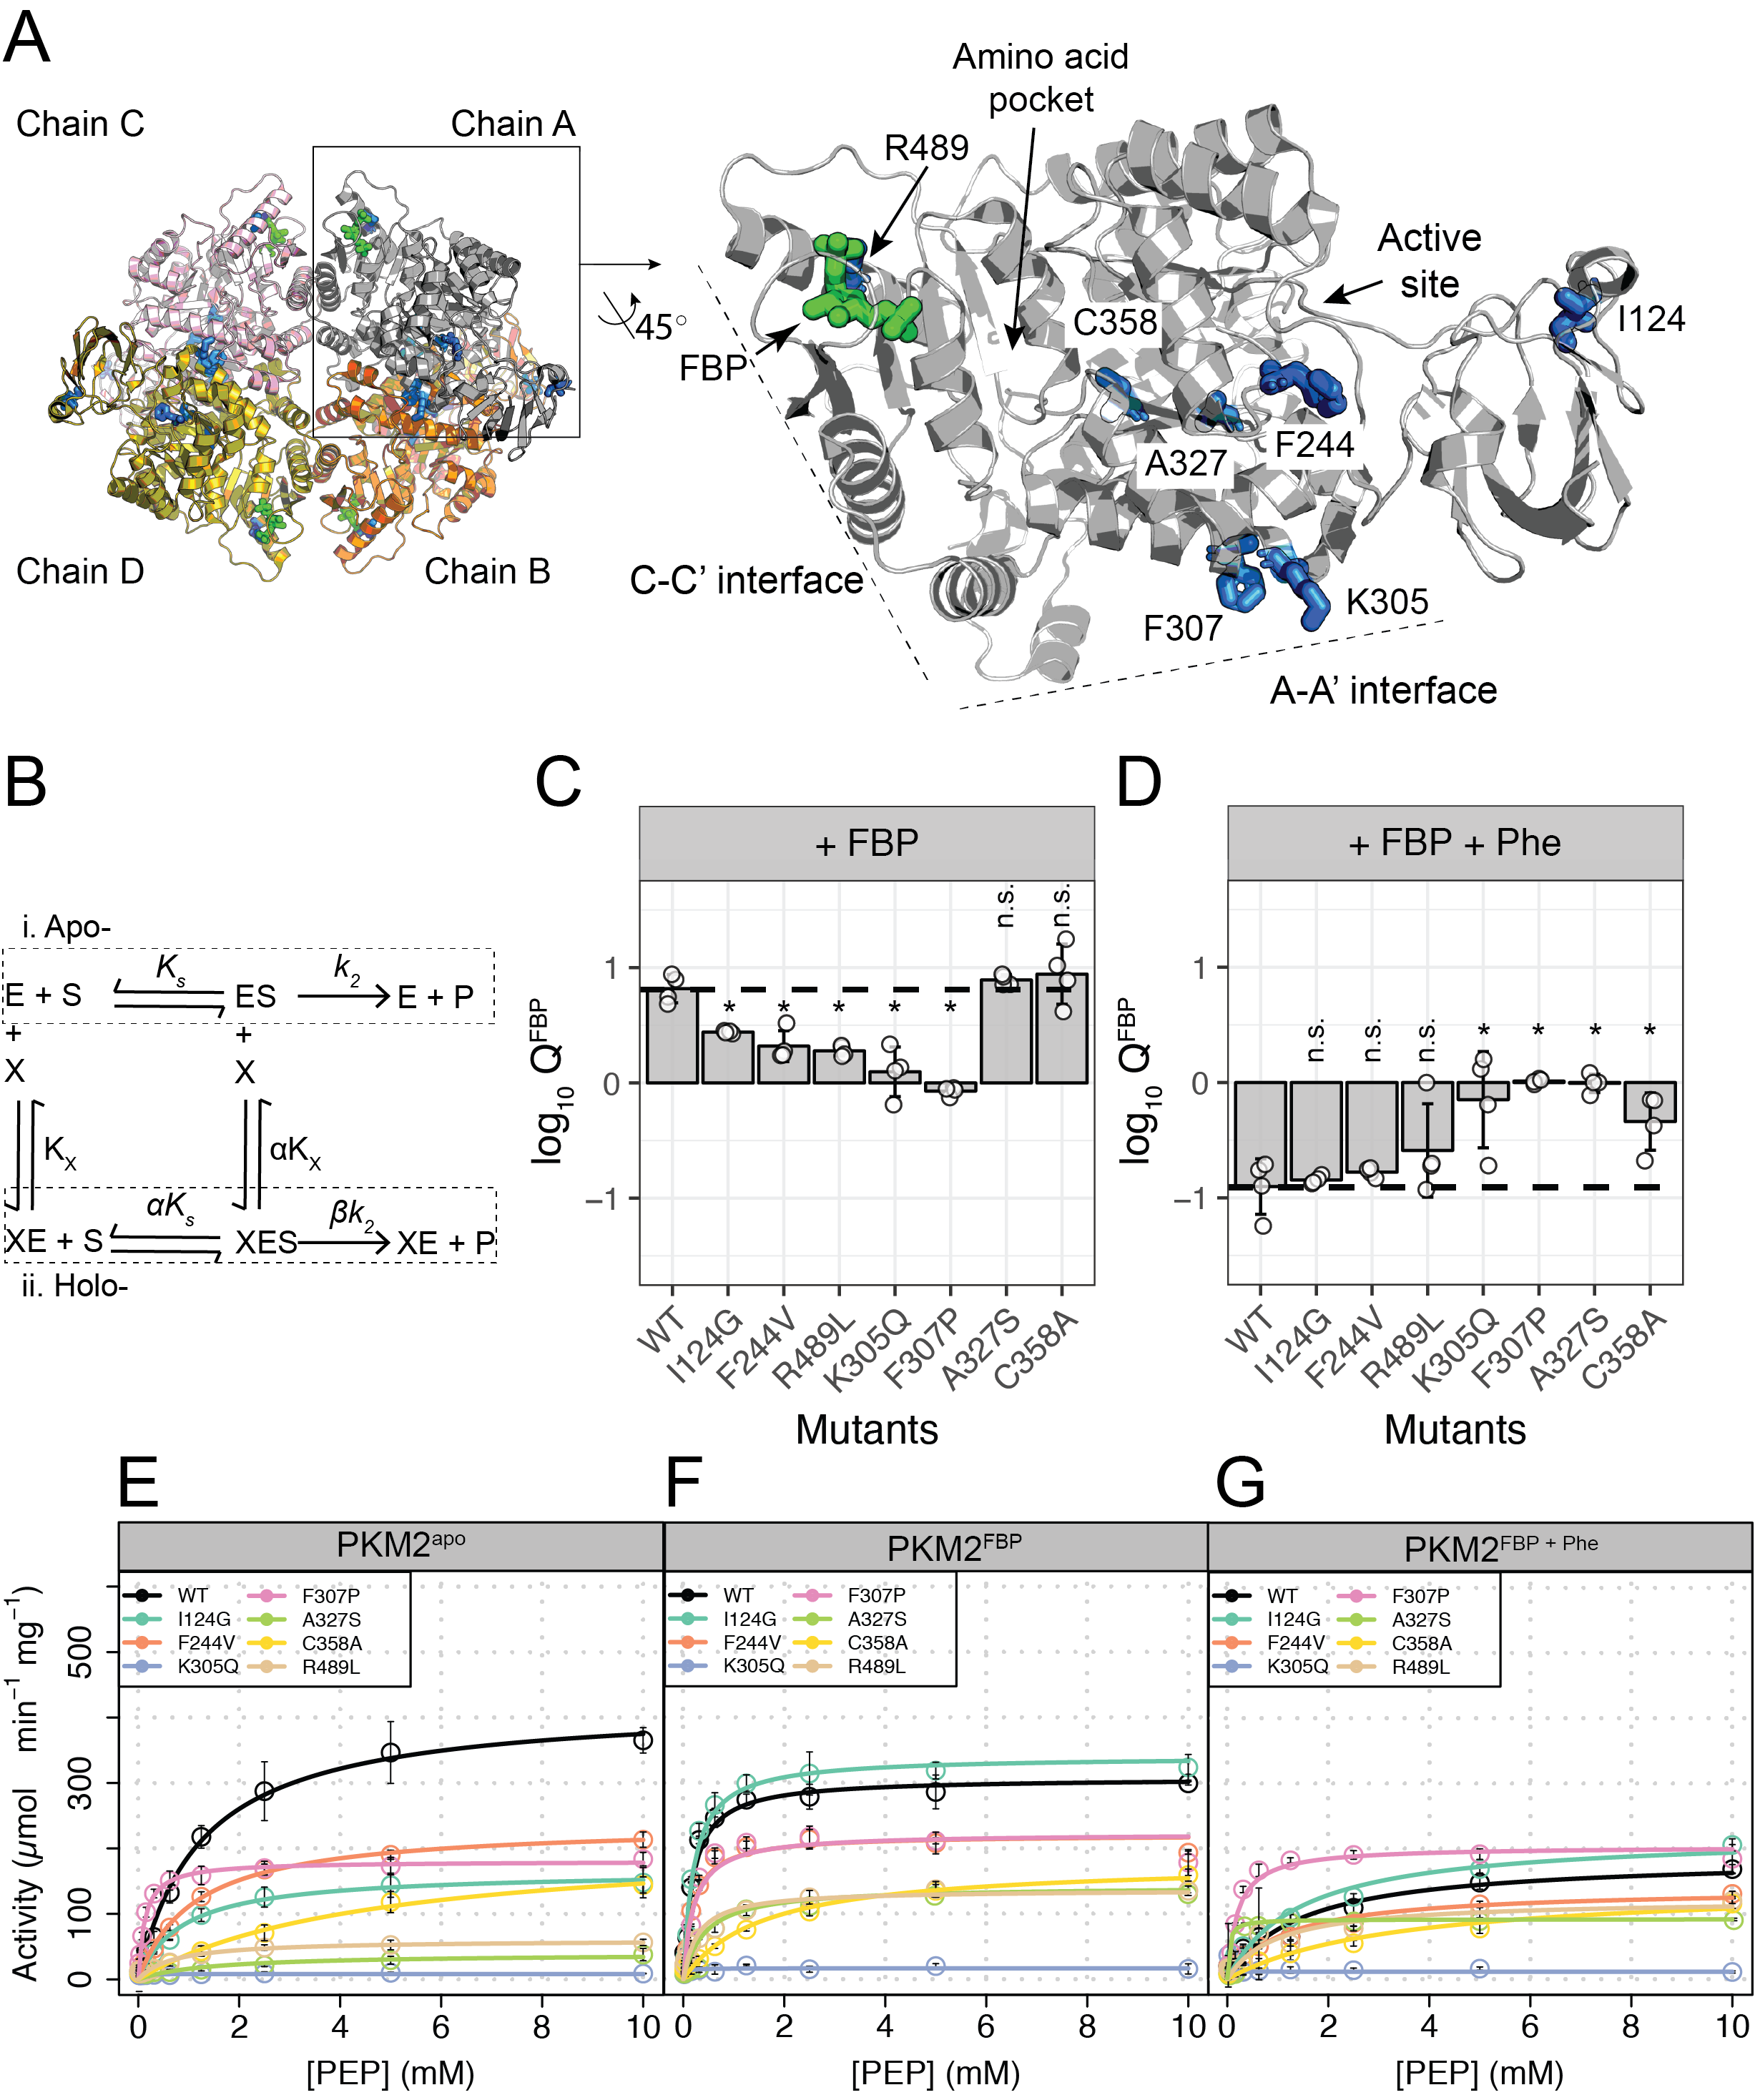
\includegraphics[scale=0.6]{ch7_fig6_apo_fbp_rate_curves.png}
\caption[The AlloHubMuts perturb either FBP-active site coupling or FBP-Phe coupling.] {\textbf{The AlloHubMuts perturb either FBP-active site coupling or FBP-Phe coupling.} \textbf{(A)} A structural schematic showing the locations of the AlloHubMuts on PKM2 protomer. \textbf{(B)} A single-substrate-single-modifier scheme was used to quantify the coupling co-efficient ($Q$) between FBP and substrate binding and between FBP \textit{and} Phe and substrate binding. \textbf{(C)} The allosteric response of PKM2(WT) and AlloHubMuts to FBP, quantified by the allosteric coefficient, which denotes the change of the K$_{M}^{PEP}$ upon addition of saturating concentrations of FBP (see Methods Section \ref{methods:coupling_coef}). The Q-coefficient for wild type PKM2 (WT) is shown as a dotted line for comparison. Each of the Q-coefficients of the AlloHubMuts were statistically compared to PKM2(WT) using a Wilcoxon ranked-sum test (n = 4); a p-value < 0.05 was deemed significant (denoted by an asterisk); n.s.: not significant. \textbf{(D)} The magnitude of allosteric inhibition by Phe, in the presence of FBP, determined for PKM2(WT) and AlloHubMuts, quantified by the allosteric co-efficient Q as in (B). Raw initial velocity rate curves are shown in the absence of added ligands in \textbf{(E)}, in the presence of saturating FBP \textbf{(F)} and in the presence of saturating FBP and 400 $\mu$M Phe \textbf{(G)}.}
\label{fig:fbp_coupling_constant}
\end{figure}
%
%
\clearpage
%
%
%%%TABLE
% Please add the following required packages to your document preamble:
% \usepackage{booktabs}
\begin{table}[!ht]
\centering
\caption[Steady-state enzyme kinetic parameters of the AlloHubMuts.]{\textbf{Steady-state enzyme kinetic parameters of the AlloHubMuts.} The enzyme activity of the AlloHubMuts were measured over a range of phosphoenolpyruvate concentrations between 0 mM and 10 mM in the absence of added ligands, in the presence of saturating concentrations of FBP and in the presence of FBP and 400 $\mu$M (physiological concentrations) Phe. A protein concentration of 5 nM was used for all measurements. Activity measurements were repeated four times; the mean and standard deviations are shown.}
\begin{tabular}{@{}lllll@{}}
\toprule
AlloHubM & Ligand & K$_{M}^{PEP}$ (mM) & k$_{cat}$ (s$^{-1}$) & k$_{cat}$/K$_{M}^{PEP}$ (s$^{-1}\cdot$ mM$^{-1}$) \\ \midrule
I124G & Apo & 1.07 $\pm$ 0.13 & 190.27 $\pm$ 7.31 & 177.82 $\pm$ 56.23 \\
 & FBP & 0.29 $\pm$ 0.04 & 307.10 $\pm$ 6.11 & 1058.97 $\pm$ 152.75 \\
 & FBP+Phe & 1.44 $\pm$ 0.34 & 221.92 $\pm$ 17.26 & 153.98 $\pm$ 37.88 \\\midrule
F244V & Apo & 1.14 $\pm$ 0.11 & 237.44 $\pm$ 7.36 & 210.44 $\pm$ 27.15 \\
 & FBP & 0.55 $\pm$ 0.07 & 279.62 $\pm$ 9.93 & 522.42 $\pm$ 87.51 \\
 & FBP+Phe & 1.15 $\pm$ 0.30 & 222.51 $\pm$ 18.29 & 195.87 $\pm$ 55.46 \\\midrule
K305Q & Apo & 0.01 $\pm$ 0.01 & 8.06 $\pm$ 0.57 & 790.01 $\pm$ 605.56 \\
 & FBP & 0.01 $\pm$ 0.04 & 8.40 $\pm$ 0.43 & 1038.01 $\pm$ 535.50 \\
 & FBP+Phe & 0.04 $\pm$ 0.01 & 12.21 $\pm$ 1.40 & 408.37 $\pm$ 136.10 \\\midrule
F307P & Apo & 0.13 $\pm$ 0.01 & 180.47 $\pm$ 3.05 & 1413.87 $\pm$ 133.12 \\
 & FBP & 0.15 $\pm$ 0.02 & 227.20 $\pm$ 5.02 & 1508.53 $\pm$ 190.71 \\
 & FBP+Phe & 0.21 $\pm$ 0.03 & 328.71 $\pm$ 12.37 & 1568.32 $\pm$ 268.58 \\\midrule
A327S & Apo & 1.37 $\pm$ 0.42 & 31.8 $\pm$ 2.43 & 23.21 $\pm$ 5.79 \\
 & FBP & 0.17 $\pm$ 0.02 & 119.01 $\pm$ 6.86 & 700.06 $\pm$ 343.00 \\
 & FBP+Phe & 0.15 $\pm$ 0.02 & 100.19 $\pm$ 5.32 & 667.93 $\pm$ 266.00 \\\midrule
C358A & Apo & 4.71 $\pm$ 0.99 & 214.73 $\pm$ 21.40 & 45.59 $\pm$ 21.62 \\
 & FBP & 0.58 $\pm$ 0.18 & 191.13 $\pm$ 16.22 & 329.53 $\pm$ 90.11 \\
 & FBP+Phe & 1.25 $\pm$ 0.07 & 199.01 $\pm$ 21.87 & 159.20 $\pm$ 31.24 \\\midrule
R489L & Apo & 0.69 $\pm$ 0.19 & 60.05 $\pm$ 4.91 & 89.38 $\pm$ 36.93 \\
 & FBP & 0.36 $\pm$ 0.10 & 112.25 $\pm$ 7.60 & 317.20 $\pm$ 125.71 \\
 & FBP+Phe & 1.44 $\pm$ 0.40 & 132.99 $\pm$ 15.74 & 158.19 $\pm$ 122.56 \\ \bottomrule
\end{tabular}
\label{tab:allohubmut_activity}
\end{table}

\clearpage


\subsection{Native spectra of AlloHubMut uncouples oligomerisation from allosteric activation}
\label{subsec:allohubmut_ms}
Native spectra of PKM2(WT), in Chapter \ref{chapter:mass_spec}, showed that FBP-induced allosteric activation is accompanied by stabilisation of the high-substrate affinity tetrameric state. This observation led to the hypothesis that tetramerisation and enzyme activation are coupled. It would be expected, therefore, that a mutant which prevents tetramer formation would reveal a reduced (or no) allosteric response to FBP, prompting the lack of oligomerisation as a possible explanation as to why some of the AlloHubMuts had a reduced coupling between the FBP pocket and the active site (Sections \ref{subsec:allohubmuts_fbp} and \ref{subsec:allohubmuts_phe}).
%
%
\\\\
%
%
To this end, native spectra of the AlloHubMuts were acquired in the absence of any added ligands (\textbf{Fig. \ref{fig:allohubmut_ms} A}), and following pre-incubation with FBP at a ratio of 2:1 (ligand-to-protein) (\textbf{Fig. \ref{fig:allohubmut_ms} B}). A327S and C358A both formed of monomers, dimers and tetramers, at an approximate ratio of 1:3:6 (\textbf{Fig. \ref{fig:allohubmut_ms} C}). The addition of FBP to A327S and C358A resulted in a complete conversion of lower-order oligomers into tetramers, similar to PKM2(WT) (\textbf{Fig. \ref{fig:allohubmut_ms} C}). In contrast, F244V and R489L formed monomer-dimer-tetramer equilibria, both at approximate ratios of 1:3:6, which was unperturbed following the addition of FBP (\textbf{Fig. \ref{fig:allohubmut_ms} C}). The oligomeric response of A327S and C358A and the lack of response of F244V and R489L fit with the previous observation that A327S and C358A maintain an intact allosteric coupling between the FBP pocket and the active site, and that F244V and R489L have a significantly reduced enzymatic response to FBP (Section \ref{subsec:allohubmuts_fbp}). 
%
%
\\\\
%
%
PKM2(I124G) formed a monomer-dimer-tetramer mixture, in the absence of added ligands, at an ratio equivalent to that of the wild-type (\textbf{Fig. \ref{fig:allohubmut_ms} C}). The addition of FBP to I124G resulted in an apparent tetramerisation, despite the observation that this mutant has a significantly reduced enzymatic response to FBP binding. Conversely, K305Q exclusively formed monomers in the absence of FBP, likely due to the removal of a charged interaction between K305 and E384 at the A-A' interface (\textbf{Fig. \ref{fig:unfolding_apo} H}). Nevertheless, the addition of FBP to K305Q resulted in the formation of a significant fraction of tetramers, with a monomer-dimer-tetramer distribution of approximately 4:1:5 (\textbf{Fig. \ref{fig:allohubmut_ms}}). Taken together, the finding that I124G and K305Q undergo an apparent tetramerisation upon FBP addition, despite the negated coupling between the FBP pocket and the active site, provided evidence to suggest that PKM2 allosteric activation is uncoupled from oligomerisation. 
%
%
%
%
%%% FIGURE
%
\begin{figure}[!ht]
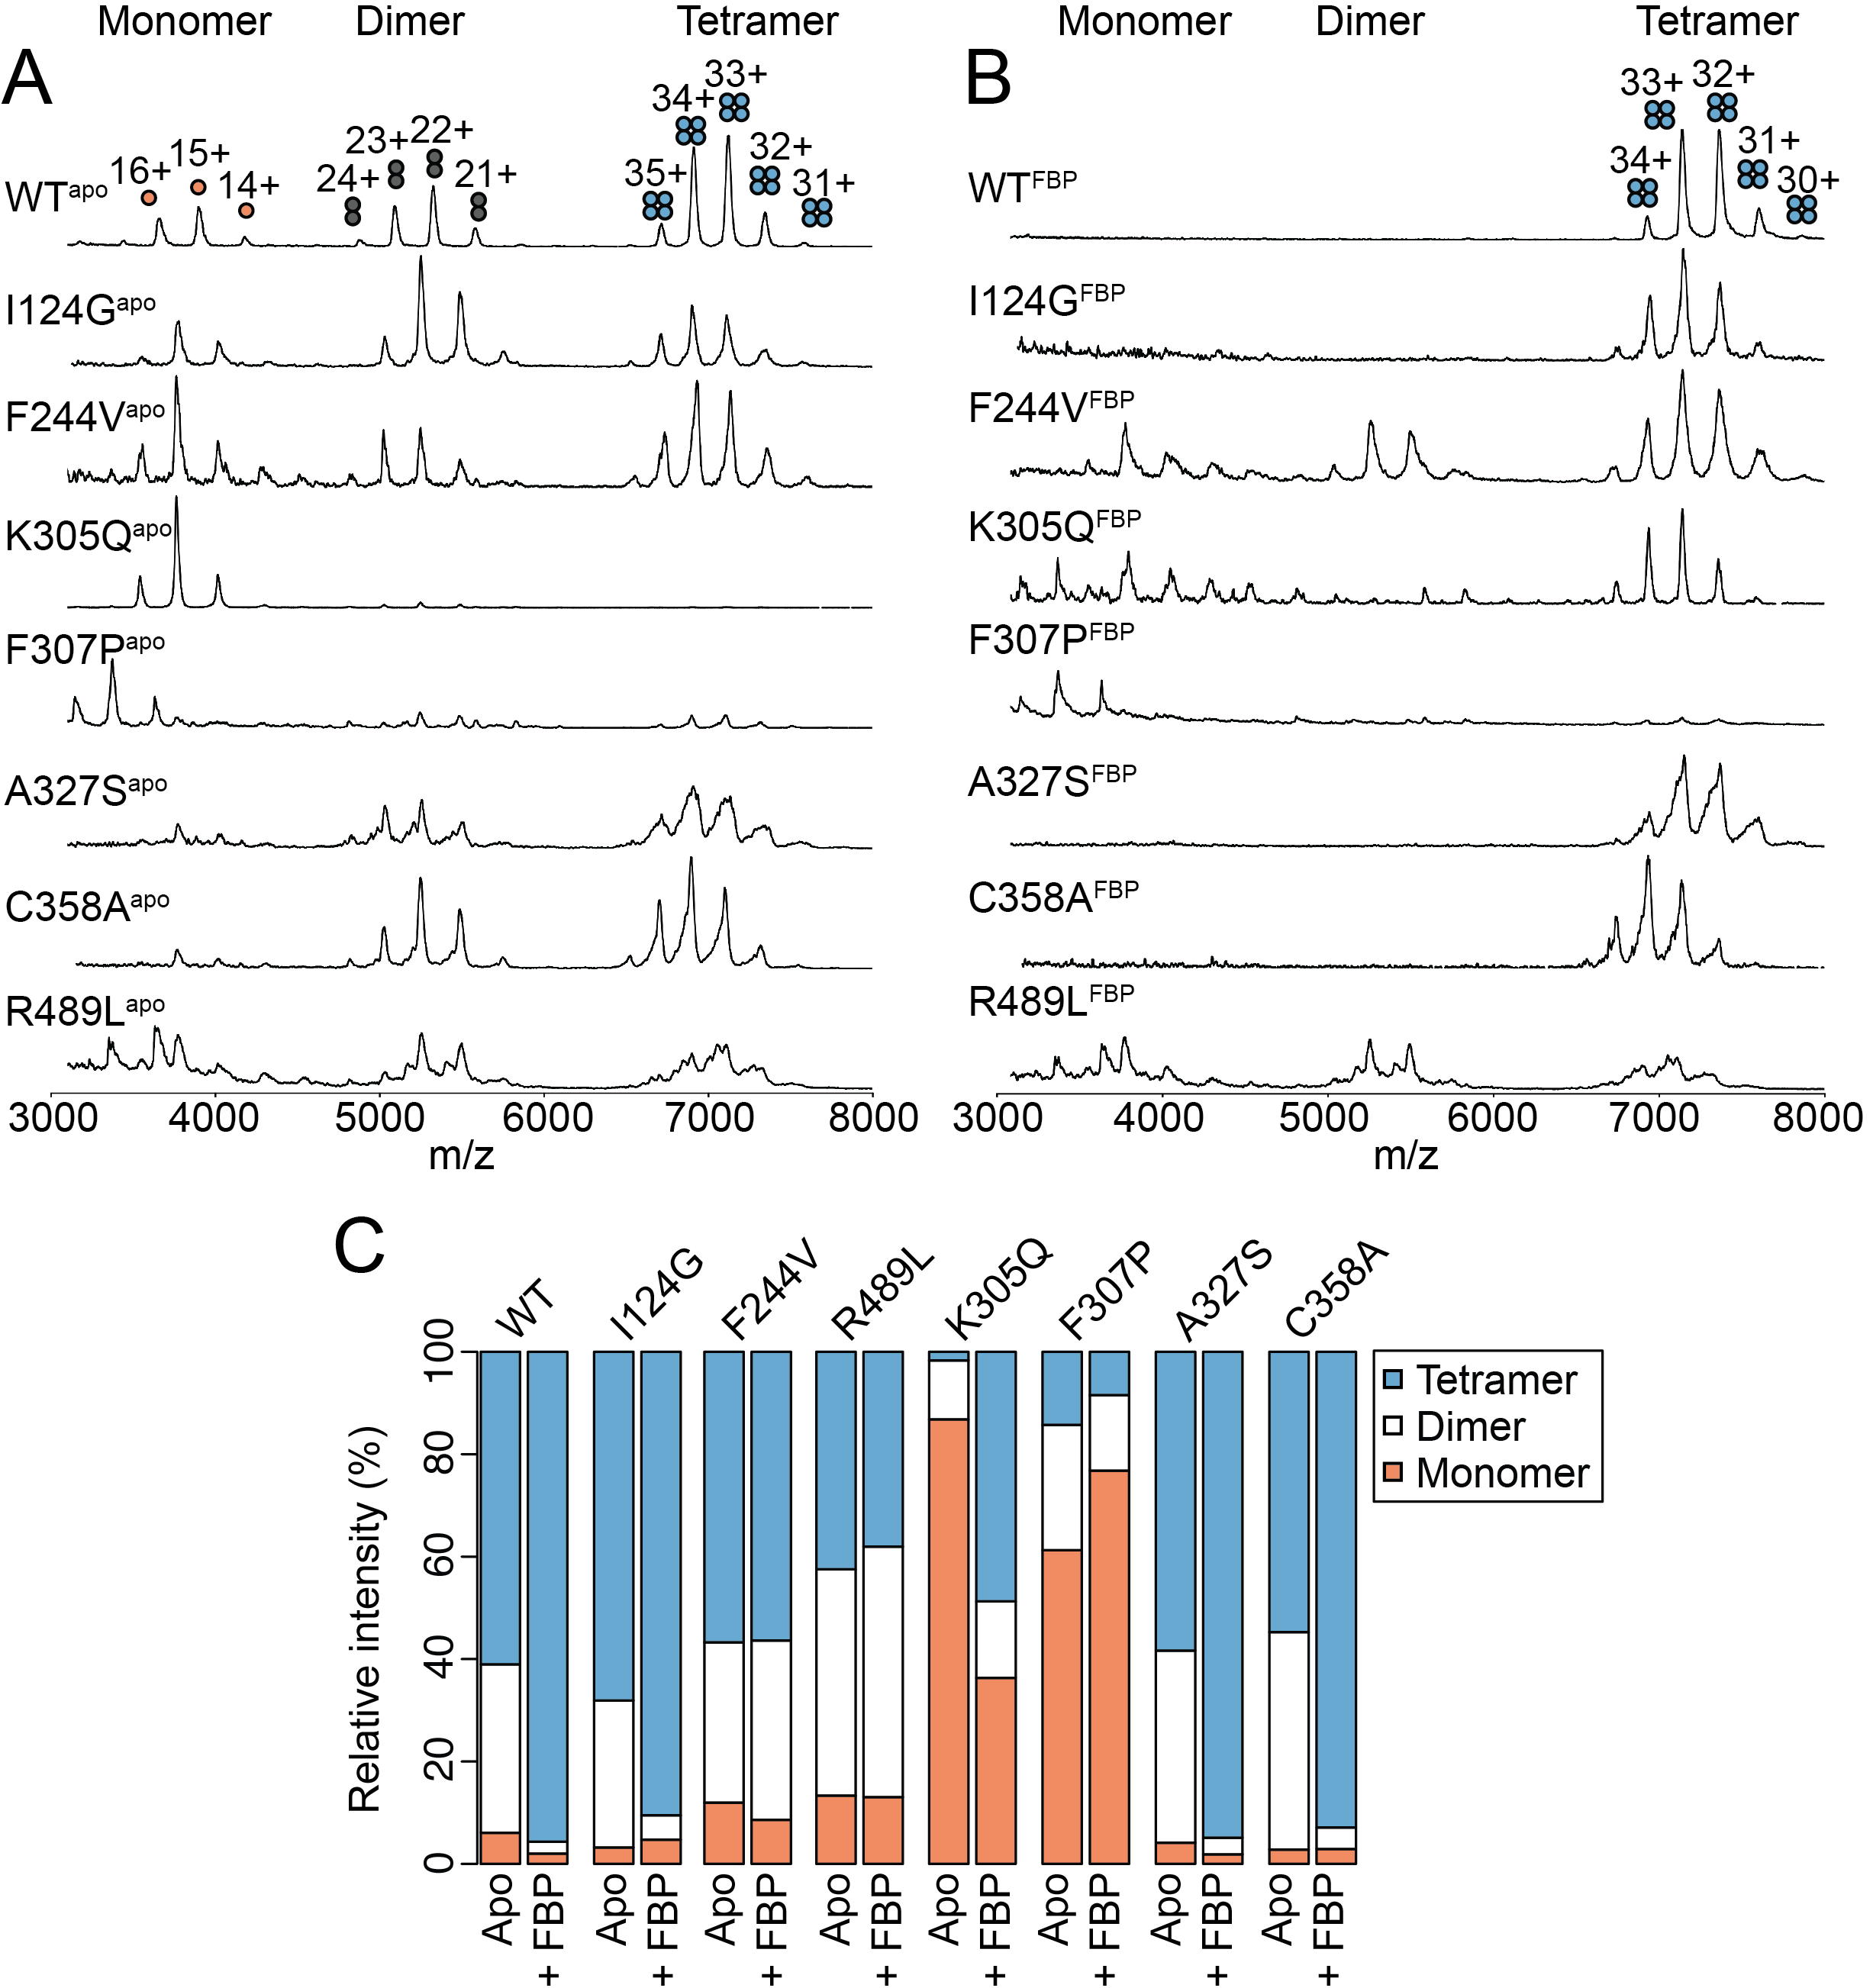
\includegraphics[scale=0.7]{ch7_fig8_muts_nMS.png}
\caption[Native spectra of the AlloHubMuts reveal a complex relationship between allosteric activation and oligomerisation.] {\textbf{Native spectra of the AlloHubMuts reveal a complex relationship between allosteric activation and oligomerisation.} Nano-electrospray ionisation mass spectrometry was used to acquire native spectra of \textbf{(A)} PKM2(WT) and the AlloHubMuts, individually in the absence of added ligands and \textbf{(B)} in the presence of FBP. PKM2 variants were pre-incubated with FBP at a ratio of (2:1; protein-to-ligand). \textbf{(C)} The oligomeric state distribution was quantified for each of the AlloHubMuts and presented as stacked bars showing the relative intensities of monomers (orange), dimers (white) and tetramers (blue).}
\label{fig:allohubmut_ms}
\end{figure}
%
%
\clearpage



\section{Conclusion}
In summary, evaluation of the allosteric properties of AlloHubMuts demonstrated that a novel computational method \textit{AlloHubMat} identified residues involved in FBP-induced allostery. Two of the AlloHubMuts were found not to response to FBP \textit{per se}, but rather to attenuate Phe-induced disruption of allosteric activation by FBP, revealing two residues (A327 and C358) that mediate a functional cross-talk between allosteric networks elicited from distinct ligand binding pockets on PKM2. 










